\documentclass[a4paper, 11pt]{article}
\usepackage[english]{babel}
\usepackage{fullpage}

\usepackage[pdftex]{graphicx}
\graphicspath{{../pdf/}{../jpeg/}}
\DeclareGraphicsExtensions{.pdf,.jpeg,.png}

% ----------------------------------------------

% Definitions of languages: ------------
\usepackage{listings}
\lstdefinestyle{cStyle}{
  basicstyle=\scriptsize,
  breakatwhitespace=false,
  breaklines=true,
  captionpos=b,
  keepspaces=true,
  numbersep=5pt,
  showspaces=false,
  gobble=4,
  tabsize=4,
  showstringspaces=false,
  showtabs=false,
}
\renewcommand*{\lstlistingname}{Code}

% ----------------------------------------------

\begin{document}

\noindent
\large\textbf{CES-27 Distributed Processing} \\
\textbf{1th Activity} \\
\normalsize Prof Hirata and Prof Juliana  \\
Carlos Matheus Barros da Silva \hfill August 2019

\section*{Task 1}

It was implemented a Lamport's \textit{Scalar Logic Clock} simulation. The implementation was made in Go and it can be seen on the Repository\footnote{https://github.com/CarlosMatheus/CES-27/tree/master/lab01}.

\subsection*{Suggested Test Case}

As It was suggested, it was conducted a test with 3 terminal windows, on each one was opened one task of the program as shown in the Code \ref{code_code1}.

The test was made according to the model represented on Figure \ref{img_task1}. The results can be seen on the outputs on the

\begin{figure}[h]
  \begin{center}
  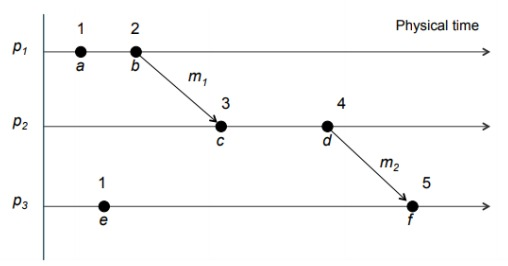
\includegraphics[width=4in]{./imgs/scalar.jpeg}
  \caption{Model representing the execution of Task 1 example test case}
  \label{img_task1}
  \end{center}
\end{figure}

\lstinputlisting[
    language=python,
    caption={Code that was run on each of the 3 terminal window on the execution of Task 1 example test case},
    label={code_code1},
    style=cStyle,
]{./code1.txt}

\begin{figure}[h]
  \begin{center}
  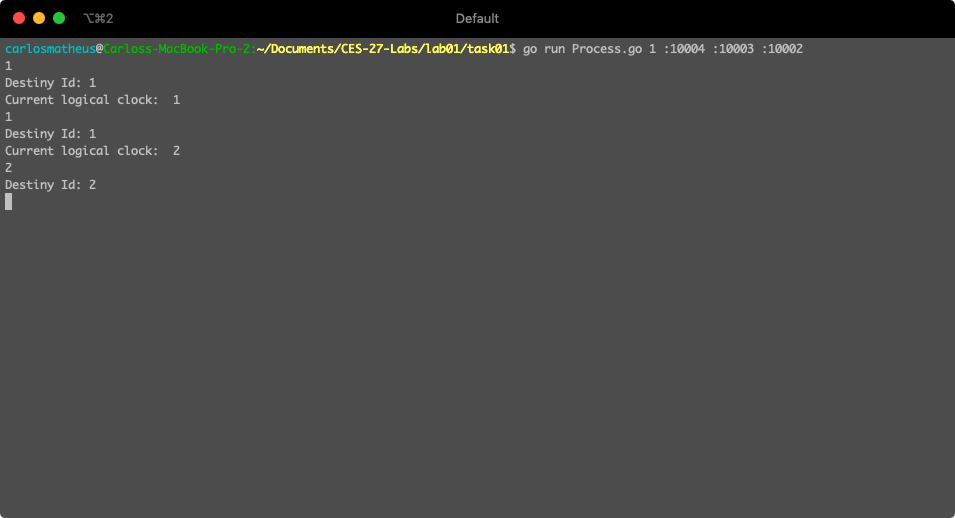
\includegraphics[width=5in]{./imgs/example_task1_window1.png}
  \caption{Window 1 after execution of Task 1 example test case}
  \label{img_example_task1_window1}
  \end{center}
\end{figure}

\begin{figure}[h]
  \begin{center}
  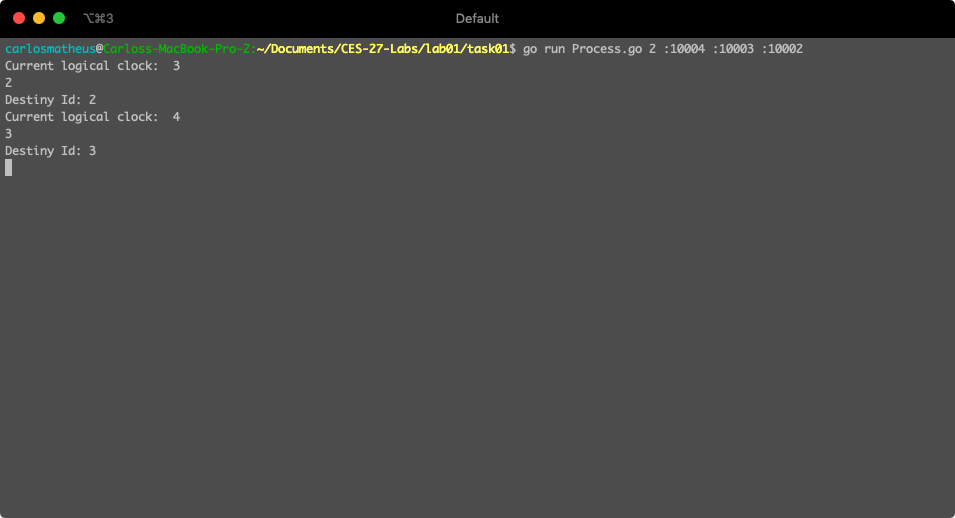
\includegraphics[width=5in]{./imgs/example_task1_window2.png}
  \caption{Window 2 after execution of Task 1 example test case}
  \label{img_example_task1_window2}
  \end{center}
\end{figure}

\begin{figure}[h]
  \begin{center}
  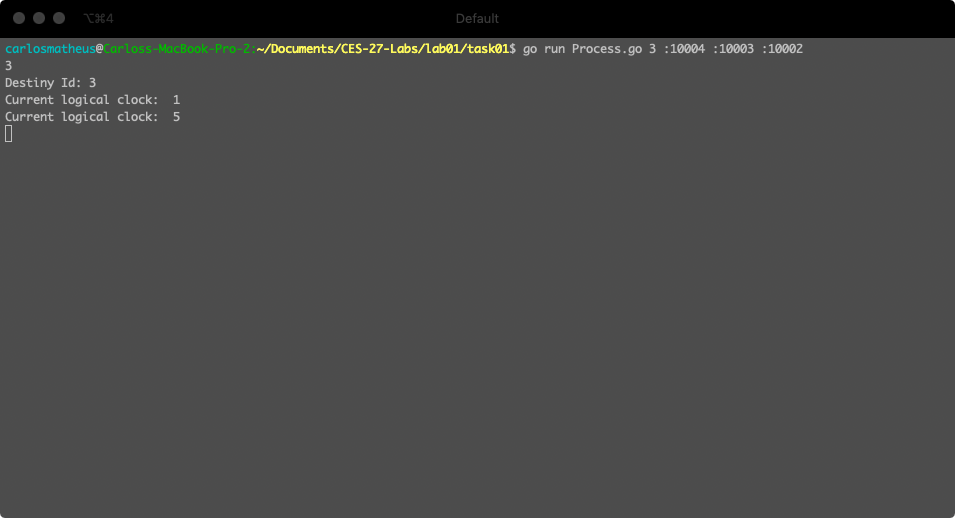
\includegraphics[width=5in]{./imgs/example_task1_window3.png}
  \caption{Window 3 after execution of Task 1 example test case}
  \label{img_example_task1_window3}
  \end{center}
\end{figure}

\subsection*{Built Test Case}

\subsection*{Research}

\begin{itemize}
    \item Explore the \textit{Stem Torproject}\cite{stem} website.
    \item Do \textit{Stem Torproject} tutorials.
    \item Look for other soucers about Tor Python libraries, including \textit{Youtube} tutorials.
\end{itemize}

\subsection*{Implementation}

Have a Python application that includes at least the following items:

\begin{itemize}
    \item Establish Tor internet connection with Python.
    \item Fetch websites with Tor connection.
    \item Create message system between two points with Tor connection.
\end{itemize}

\section*{Tor Android App}

This section is extra to this project. Once the first part related to the Python application is done, the focus will be to try to make the same kind of application to run on an Android.

\subsection*{Research}

\begin{itemize}
    % \item Explore the \textit{NetCipher}\cite{netcipher} Repository.
    \item Study \textit{OrbotHelper} class in \textit{Stem Torproject}\cite{stem}.
\end{itemize}

\subsection*{Implementation}

\begin{itemize}
    \item Adapt the Python application to work on Android.
\end{itemize}

\section*{Initial Schedule}

\begin{itemize}
    \item March: Study on Python Tor Libraries.
    \item April: Develop Python app.
    \item May: Study Android Tor app Library. Start Tor app implementation.
    \item June: Finish Tor app implementation. Write the report. Make the project presentation.
\end{itemize}

\newpage
\bibliographystyle{plain}
\bibliography{bibliography.bib}

\end{document}
